\documentclass[]{article}
\usepackage{graphicx}
\usepackage{enumitem}
\usepackage{amsmath,amsthm,amssymb}

\title{BMI Mathe 3: Stochastik Uebungsaufgaben}
\author{M.Sc. Marcel Tiator}

\begin{document}

\maketitle
	
\section{Beispiel 1.21}

In einem Restaurant bestellen gewöhnlich $40\%$ der Gäste keine Vorspeise und der $30\%$ der Gäste keine Nachspeise. $15\%$ der Gäste nehmen weder eine Vorspeise noch eine Nachspeise. Wie groß ist die Wahrscheinlichkeit, dass

\begin{enumerate}[label=\alph*)]
	\item ein Gast keine Nachspeise nimmt, unter der Bedingung, dass er auch keine Vorspeise genommen hat?
	\item ein Gast, der eine Vorspeise gewählt hat, auch noch eine Nachspeise nimmt? 
\end{enumerate}

\subsection{Loesung a)}

Sei $N$ das Ereignis der Wahl einer Nachspeise und $V$ das Ereignis der Wahl einer Vorspeise. 

\begin{equation}
	\begin{split}
		ges.: & P(\overline{N} \vert \overline{V}) \\
		geg.: & P(\overline{N} \vert \overline{V}) = \frac{P(\overline{N} \cap \overline{V})}{P(\overline{V})} \\
		& P(\overline{V}) = 0.4 \\
		& P(\overline{N} \cap \overline{V}) = 0.15 \\
		& \\
		& P(\overline{N} \vert \overline{V}) = \frac{P(\overline{N} \cap \overline{V})}{P(\overline{V})} = \frac{0.15}{0.4} = 0.375
	\end{split}
\end{equation}

\subsection{Loesung b)}

Sei $N$ das Ereignis der Wahl einer Nachspeise und $V$ das Ereignis der Wahl einer Vorspeise. 

\begin{equation}
	\begin{split}
		ges.: & P(N \vert V) \\
		geg.: & P(N \vert V) = \frac{P(N \cap V)}{P(V)} \\
		& P(V) = 1 - P(\overline{V}) = 1 - 0.4 = 0.6 \\
		& P(N) = 1 - P(\overline{N}) = 1 - 0.3 = 0.7 \\
		& P(N \cap V) = P(N) + P(V) - P(N \cup V) \\
		& \\
		& P(N \cup V) = 1 - P(\overline{N \cup V}) \\
		& P(\overline{N \cup V}) = P(\overline{N} \cap \overline{V}) = 0.15 \\
		& P(N \cup V) = 1 - P(\overline{N \cup V}) = 1 - 0.15 = 0.85 \\
		& \\
		& P(N \cap V) = 0.6 + 0.7 - 0.85 = 0.45 \\
		& \\
		& P(N \vert V) = \frac{P(N \cap V)}{P(V)} = \frac{0.45}{0.6} = 0.75
	\end{split}
\end{equation}

\section{Aufgabe $27$}

Die Trompeter Andreas, Berti und Christoph lassen in ihrem Musikverein den Zufall bestimmen, wer die solistischen Stellen zu spielen hat. Dazu wuerfeln sie vor dem Stueck einmal mit einem fairen Wuerfel. Andreas spielt das Solo, wenn eine $1$ faellt, Berti bei einer $2$ oder $3$, Christoph schließlich bei $4$, $5$ oder $6$. \\
Andreas spielt Solostellen mit einer Wahrscheinlichkeit von $80\%$ perfekt (mit einer Wahrscheinlichkeit von $20\%$ ist mindestens ein schraeger Ton dabei), Berti spielt Soli mit einer Wahrscheinlichkeit von $90\%$ perfekt, Christoph mit einer Wahrscheinlichkeit von $95\%$. 

\begin{enumerate}[label=\alph*)]
	\item Mit welcher Wahrscheinlichkeit wird ein Trompetensolo perfekt zu Gehoer gebracht? 
	\item Bei einem Solo war deutlich ein falscher Ton zu hoeren. Mit welcher Wahrscheinlichkeit hat Berti das Solo gespielt? 
\end{enumerate}

\subsection{Loesung a)}

Sei $S$ das Ereignis des Spielens eines Solos. Sei $W_1$ das Wuerfeln der Augenzahl $1$. Sei $W_2$ das Wuerfeln der Augenzahlen $2, 3$ und $W_2$ das Wuerfeln der Augenzahlen $4, 5, 6$. 

\begin{equation}
	\begin{split}
		ges.: P(S) & \\
		geg.: P(S) &= \underset{i=1}{\overset{3}{\mathrm{\sum}}} P(S \vert W_i) \cdot P(W_i)\\
		W_1 &= \{1\} \\
		W_2 &= \{2, 3\} \\
		W_3 &= \{4, 5, 6\} \\
		\Omega &= \{1, 2, 3, 4, 5, 6\} \\
		P(S \vert W_1) &= 0.8 \\
		P(S \vert W_2) &= 0.9 \\
		P(S \vert W_3) &= 0.95 \\
		& \\
		P(W_1) &= \frac{\vert W_1 \vert}{\vert \Omega \vert} = \frac{1}{6} \\
		P(W_2) &= \frac{2}{6} = \frac{1}{3} \\
		P(W_3) &= \frac{3}{6} = \frac{1}{2} \\
		& \\
		P(S) &= P(S \vert W_1) \cdot P(W_1) + P(S \vert W_2) \cdot P(W_2) + P(S \vert W_3) \cdot P(W_3) \\
		&\approx 0.908
	\end{split}
\end{equation}

\subsection{Loesung b)}

\begin{equation}
	\begin{split}
		ges.: & P(W_2 \vert \overline{S}) \\
		geg.: & P(W_2 \vert \overline{S}) = \frac{P(\overline{S} \vert W_2) \cdot P(W_2)}{P(\overline{S})} \\
		& \\
		P(\overline{S}) &= 1 - P(S) = 1 - 0.908 = 0.092 \\
		P(\overline{S} \vert W_2) &= 1 - P(S \vert W_2) = 1 - 0.9 = 0.1 \\
		P(W_2 \vert \overline{S}) &\approx 0.362
	\end{split}
\end{equation}

\section{Verstaendnisaufgabe Rechenregeln 1}

$P(A) + P(\overline{A})$ is gleich?

\begin{enumerate}[label=\alph*)]
	\item $P(A \cup \overline{A})$
	\item $P(\Omega)$
	\item $P(\emptyset)$
	\item $1$
\end{enumerate}

\subsection{Loesung}

a), b), d)

\section{Verstaendnisaufgabe Rechenregeln 2}

Ist folgende Aussage wahr? $P(A) \geq P(B)$ falls $A \subseteq B$.

\subsection{Loesung}

Die Aussage ist falsch. 
\begin{equation}
	\begin{split}
		A \subseteq B \iff B & = A \cup (B \setminus A) \\
		P(B) & = P(A) + P(B \setminus A) \\
		\text{daher ist } & P(B) \geq P(A) 
	\end{split}
\end{equation}

\begin{figure}[h]
	\centering
	\includegraphics[width=0.25\columnwidth]{./verstaendnis_2/veranschaulichung.png}
\end{figure}

\section{Verstaendnisaufgabe Rechenregeln 3}

Ordnen Sie die folgenden Aussagen den entsprechenden Termen zu:

\begin{enumerate}[label=\alph*)]
	\item Es passiert $A$ oder $B$. 
	\item Es passiert $A$ und $B$.
\end{enumerate}

\begin{enumerate}
	\item $A \cap B$
	\item $A \cup B$
\end{enumerate}

\subsection{Loesung}

a) gehoert zu 2., b) gehoert zu 1.

\section{Verstaendnisaufgabe Rechenregeln 4}

Gegeben sind die Ereignisse A, B und C. Die Wahrscheinlichkeit des Ereignisses A oder B oder C kann folgendermaßen berechnet werden: 

\begin{enumerate}
	\item $P(A \cap B \cap C) = P(A) + P(B) + P(C) - P(A \cap B) - P(B \cap C) - P(C \cap A) + P(A \cup B \cup C)$
	\item $P(A \cup B \cup C) = P(A) + P(B) + P(C) - P(A \cap B) - P(B \cap C) - P(C \cap A)$
	\item $P(A \cap B \cap C) = P(A) + P(B) + P(C)$
	\item $P(A \cup B \cup C) = P(A) + P(B) + P(C) - P(A \cap B) - P(B \cap C) - P(A \cap C) + P(A \cap B \cap C)$ \label{item:ex4_sol}
\end{enumerate}

\subsection{Loesung}

Die richtige Antwort ist \ref{item:ex4_sol}.. Mit $P(A) + P(B) + P(C)$ haben wir die Flächen $P(A \cap B), P(B \cap C)$ und $P(A \cap C)$ zu viel berechnet, daher ziehen wir diese ab (siehe Abbildung~\ref{fig:verstaendnis_4}). Jedoch haben wir damit die Mitte geloescht, wodurch diese mit $P(A \cap B \cap C)$ wieder addieren. 

\begin{figure}
	\centering
	\includegraphics[width=0.5\columnwidth]{./verstaendnis_4/erklaerung.png}
	\label{fig:verstaendnis_4}
\end{figure}

\end{document}
